\documentclass{llncs}
\usepackage{xcolor}
\usepackage[utf8]{inputenc}
\usepackage{amssymb}
\usepackage{amsmath}
\usepackage{tikz}
\usetikzlibrary{automata, positioning, arrows}
\tikzset{
->, % makes the edges directed
>=stealth, % makes the arrow heads bold
node distance=3cm, % specifies the minimum distance between two nodes. Change if necessary.
shorten >=1pt,
every state/.style={thick, fill=gray!10}, % sets the properties for each ’state’ node
inner sep=0pt,
minimum size=0pt,
initial text=$ $, % sets the text that appears on the start arrow
}

\begin{document}

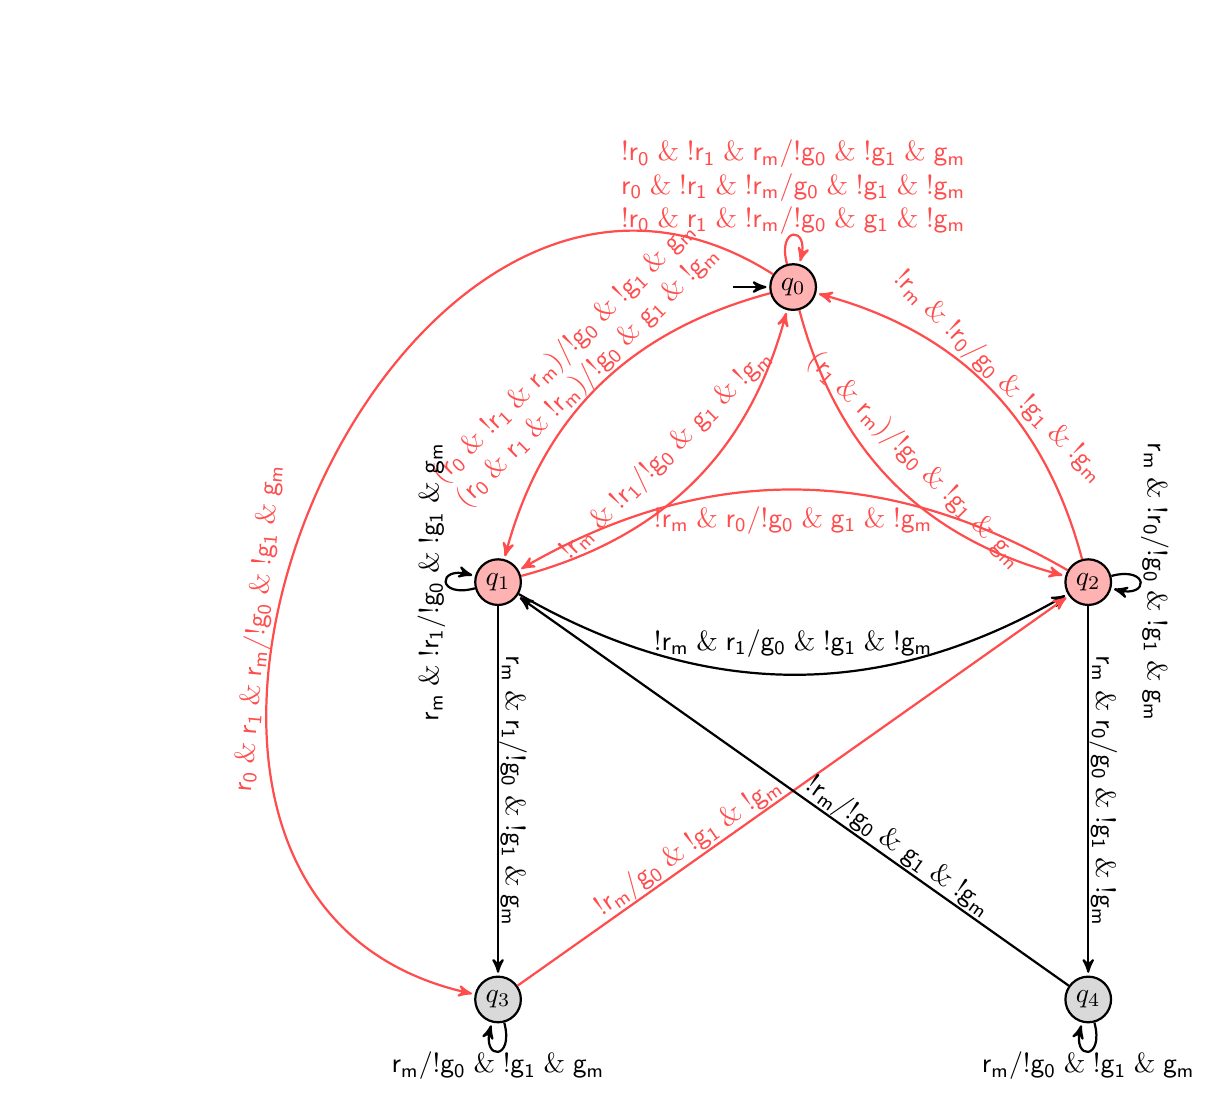
\begin{tikzpicture}[->,>=stealth',shorten >=1pt,auto,node distance=5.3cm,
                    thick,inner sep=0pt,minimum size=0pt]
  \tikzstyle{every state}=[fill=gray!30,text=black,inner
  sep=2pt,minimum size=12pt]
        \node[state, initial, fill=red!30] (q0) {$q_0$};
        \node[state, below left of=q0, fill=red!30] (q1) {$q_1$};
        \node[state, below right of=q0, fill=red!30] (q2) {$q_2$};
        \node[state, below of=q1] (q3) {$q_3$};
        \node[state, below of=q2] (q4) {$q_4$};
        \draw
            (q0) edge[loop above, align=center, color=red!70] node{$!\mathsf{r_0}\;\&\;!\mathsf{r_1}\;\&\;\mathsf{r_m}/!\mathsf{g_0}\;\&\;!\mathsf{g_1}\;\&\;\mathsf{g_m}$\\$\mathsf{r_0}\;\&\;!\mathsf{r_1}\;\&\;!\mathsf{r_m}/\mathsf{g_0}\;\&\;!\mathsf{g_1}\;\&\;!\mathsf{g_m}$\\$!\mathsf{r_0}\;\&\;\mathsf{r_1}\;\&\;!\mathsf{r_m}/!\mathsf{g_0}\;\&\;\mathsf{g_1}\;\&\;!\mathsf{g_m}$} (q0)
            (q0) edge[bend right, left, align=center, color=red!70] node[above, sloped]{$(\mathsf{r_0}\;\&\;!\mathsf{r_1}\;\&\;\mathsf{r_m})/!\mathsf{g_0}\;\&\;!\mathsf{g_1}\;\&\;\mathsf{g_m}$\\$(\mathsf{r_0}\;\&\;\mathsf{r_1}\;\&\;!\mathsf{r_m})/!\mathsf{g_0}\;\&\;\mathsf{g_1}\;\&\;!\mathsf{g_m}$} (q1)
            (q0) edge[bend right=100, looseness=1.5, left, color=red!70] node[pos=0.4, rotate=30,sloped, xshift=-1cm, yshift=1.2cm]{$\mathsf{r_0}\;\&\;\mathsf{r_1}\;\&\;\mathsf{r_m}/!\mathsf{g_0}\;\&\;!\mathsf{g_1}\;\&\;\mathsf{g_m}$} (q3)
            (q0) edge[bend right, above, color=red!70] node[above, sloped, yshift=2mm]{$(\mathsf{r_1}\;\&\;\mathsf{r_m})/!\mathsf{g_0}\;\&\;!\mathsf{g_1}\;\&\;\mathsf{g_m}$} (q2)
            (q1) edge[loop left, left] node[above, sloped]{$\mathsf{r_m}\;\&\;!\mathsf{r_1}/!\mathsf{g_0}\;\&\;!\mathsf{g_1}\;\&\;\mathsf{g_m}$} (q1)
            (q2) edge[loop right, right] node[above, sloped]{$\mathsf{r_m}\;\&\;!\mathsf{r_0}/!\mathsf{g_0}\;\&\;!\mathsf{g_1}\;\&\;\mathsf{g_m}$} (q2)
            (q1) edge[bend right, above] node[yshift=2mm]{$!\mathsf{r_m}\;\&\;\mathsf{r_1}/\mathsf{g_0}\;\&\;!\mathsf{g_1}\;\&\;!\mathsf{g_m}$} (q2)
            (q1) edge[bend right, left, color=red!70] node[above, sloped, yshift=3mm]{$!\mathsf{r_m}\;\&\;!\mathsf{r_1}/!\mathsf{g_0}\;\&\;\mathsf{g_1}\;\&\;!\mathsf{g_m}$} (q0)
            (q2) edge[bend right, below, color=red!70] node[yshift=-2mm]{$!\mathsf{r_m}\;\&\;\mathsf{r_0}/!\mathsf{g_0}\;\&\;\mathsf{g_1}\;\&\;!\mathsf{g_m}$} (q1)
            (q2) edge[bend right, right, color=red!70] node[above, sloped]{$!\mathsf{r_m}\;\&\;!\mathsf{r_0}/\mathsf{g_0}\;\&\;!\mathsf{g_1}\;\&\;!\mathsf{g_m}$} (q0)
            (q3) edge[left, color=red!70] node[above, sloped, xshift=-1.5cm]{$!\mathsf{r_m}/\mathsf{g_0}\;\&\;!\mathsf{g_1}\;\&\;!\mathsf{g_m}$} (q2)
            (q4) edge[right] node[above, sloped, xshift=1.5cm]{$!\mathsf{r_m}/!\mathsf{g_0}\;\&\;\mathsf{g_1}\;\&\;!\mathsf{g_m}$} (q1)
            (q3) edge[loop below] node{$\mathsf{r_m}/!\mathsf{g_0}\;\&\;!\mathsf{g_1}\;\&\;\mathsf{g_m}$} (q3)
            (q4) edge[loop below] node{$\mathsf{r_m}/!\mathsf{g_0}\;\&\;!\mathsf{g_1}\;\&\;\mathsf{g_m}$} (q4)
            (q1) edge[left] node[above, sloped]{$\mathsf{r_m}\;\&\;\mathsf{r_1}/!\mathsf{g_0}\;\&\;!\mathsf{g_1}\;\&\;\mathsf{g_m}$} (q3)
            (q2) edge[right] node[above, sloped]{$\mathsf{r_m}\;\&\;\mathsf{r_0}/\mathsf{g_0}\;\&\;!\mathsf{g_1}\;\&\;!\mathsf{g_m}$} (q4);
    \end{tikzpicture}

\end{document}